\documentclass[a4paper,10pt]{article}
\usepackage[utf8x]{inputenc}
\usepackage{graphicx}
%opening
\title{}
\author{}

\begin{document}

\maketitle

\begin{abstract}

\end{abstract}

\section{Installation facile}
\subsection{Rappel}
Lors de l'obtention des sources, la compilation du projet devait se faire en ligne de commande
et ce sur chaque plateforme différente. Nous disposions néanmoins d'une base de projet pour 
\textbf{QT}. Nous avons donc du apprendre à utiliser les fonctionnalités de cette librairie
et de ses différents modules pour parvenir à prendre en main le code et commencer à y
intégrer de nouvelles fonctionnalités.

\subsection{Objectifs}
Cette façon de procéder étant tout de même lourde, il nous avait été donné comme objectif de réaliser
un installeur pour le logiciel afin de ne pas rebuter ses utilisateurs potentiels. Le but étant donc
d'avoir un livrable sur un périphérique qui soit multiplateforme et simple d'utilisation.
En effet, il avait été convenu avec les clients que la principale plateforme d'utilisation serait
MAC OS X. Celà a posé toutefois d'assez nombreux problèmes car nous n'avions ni les connaissances,
ni le matériel nécessaire à la mise en oeuvre d'un installeur sous MAC.
\\
De plus deux installeurs différents ont été demandé par plateforme, selon que la version à installer
soit destinée au professeur (version contenant l'Éditeur en plus) ou à l'élève. Ci-dessous un schéma
de l'arborescence sur le périphérique.
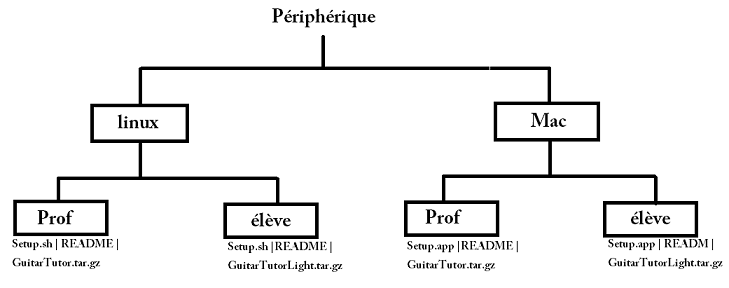
\includegraphics[scale=0.6]{arborescence_installation.png}

\subsection{Rendu}
L'installation se fait simplement par un double-clic sur une icône correspondant à l'installeur et
communique avec le client par l'intermédiaire de boîtes de dialogue. Lors de cette installation
le client doit pouvoir bénéficier des privilèges d'administrateur. Ce point nous a posé de nombreux
problèmes pour l'installation sous MAC étant donné qu'il nous est impossible de privilégier de ces
droits sur les machines de l'ENSEIRB.\\
Le premier point de l'installation est l'installation des librairies recquises, en voici la liste.\\
Pour Linux :
\begin{itemize}
 \item libqt4-dev
 \item portaudio19
 \item libsndfile1-dev
 \item libfmodex4
\end{itemize}
Et pour MAC :
\begin{itemize}
 \item qt4-base-mac-4.7.3-3
 \item portaudio18.1-3
 \item libsndfile1-dev1.0.25-1
 \item libfmodex4
\end{itemize}
Nous avions au départ opté pour une installation des librairies directement à partir des dépôts grâce
à une connexion internet. Cela permettait d'avoir une compilation et un linkage des librairies propre
et automatique. Il nous a été opposé que les dépôts n'étaient pas forcément mis à jour régulièrement
et que le client ne bénéficiait pas forcément d'une connexion internet et nous avons alors dû revoir
notre approche de l'installation. Nous avons donc dû archiver les sources des librairies et prévoir
à la fois leur compilation et leur linkage dans notre installeur. Encore une fois, nous ne pouvions
pas nous atteler à cette tâche des machines MAC de l'ENSEIRB étant donné que nous n'avions pas les 
droits.\\
\\
Ensuite on installe le logiciel en soit (selon l'installation choisie c'est à dire la version
professeur ou élève). On a un retour visuel et absolument aucune ligne de commande à taper comme
on peut le voir sur les exemples ci-dessous :\\
\\
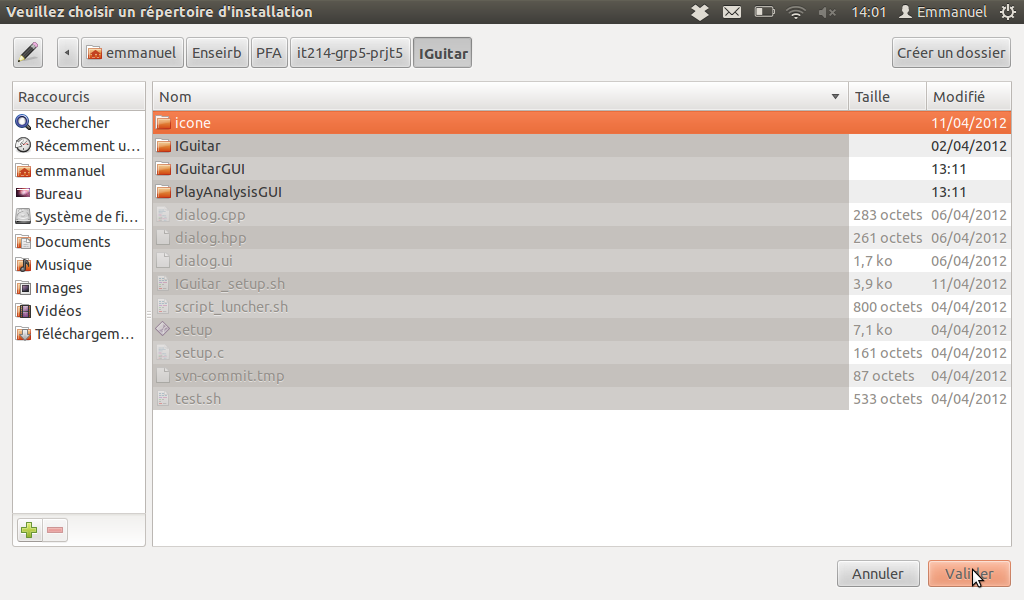
\includegraphics[scale=0.4]{./choix_repertory.png}
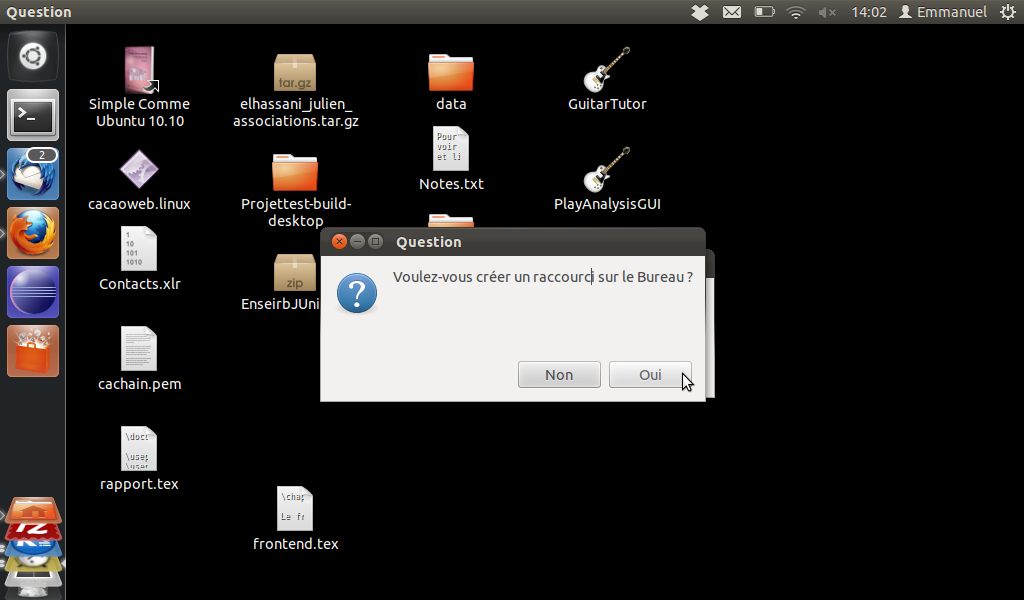
\includegraphics[scale=0.4]{./install_fin.png}

\end{document}
